\chapter{Methodology}
\label{ch:methods}

\section{Overview of the Proposed Method}

The proposed method aims to address the problem of h-index inflation by
developing three novel metrics that adjusts for the subject area and the quality
of the journal in which the publication is published. The first metric, the
\textit{Adjusted h-index} ($h_{\text{adj}}$), adjusts the h-index by only
considering publications from the top 20\% of journals in it's corresponding
subject area, based on the h5 index of the journal. The second metric, the
\textit{JIF-adjusted h-index} ($h_{\text{JIF}}$), adjusts the h-index
similarly, but the ranking of the journals is determined by the Journal Impact
Factor (JIF) of the journal in which the publication is published. Lastly, 
the \textit{Eigenfactor-adjusted h-index} ($h_{\text{EF}}$),
adjusts the h-index by considering the EigenFactor of the journal.
The proposed methods are implemented in \emph{SQL}
and the data is stored in a Sqlite database, with only the EigenFactor
calculation being done in Python.

\section{Data Collection and Preprocessing}

For the purpose of this study, the Alexandria3k \cite{Spi23g} tool was used to
collect publication data from the Crossref Dataset \cite{Crossref2020} and
prepare the data for processing. The Crossref dataset is known for its
comprehensive and standardized approach to indexing scholarly publications
across a wide range of disciplines, which is helpful for reducing discrepancies
that might arise from varying data formats used by different databases (Scopus,
Web of Science, etc.). Crossref collaborates with a large number of publishers
to ensure that a wide range of academic content is covered, including journal
articles, conference proceedings, and other scholarly works.

Alexandria3k supplies a library and a command-line tool providing efficient
relational query access to diverse publication open data sets. Specifically,
the dataset that was used is a subset of the Crossref-2024 dataset along with the subjects of
journals (from the 2024 subset) from the Crossref-2023 dataset, where the whole 
Crossref-2024 contains publication metadata from about
156 million publications from all major international publishers with full
citation data for around 60 million of them. Using our subsets we are checking
around 1.5 million publications. In addition to that, for the subject of the
publications, the Scopus ASJC (All Science Journal Classification) subject
codes were used.

To be more specific, the ASJC codes were used to categorize the publications
into more general subject areas than the original areas provided by the
Crossref-2023 dataset. The ASJC codes are a standard classification system used
to categorize publications into subject areas and are widely used in the
scientific community. The ASJC codes are hierarchical and are organized into
four levels, with the first level being the broadest and the fourth level being
the most specific. For the purpose of this study, the first level of the ASJC
codes was used to categorize the publications into subject areas, for the differentiation 
of subject areas to be differentiable. Crucial to
note is that the ASJC codes are not available for publications in the
Crossref-2024 dataset \cite{crossrefSubjectCodes2024}, so only journals with
subjects from the Crossref-2023 dataset or with subjects retrievable using the
Scopus API were considered for this study, since for those journals the ASJC
codes were able to be retrieved.

\section{Implementation of the Proposed Methods}

The proposed method was implemented in SQL using the SQLite database management
system. The implementation consists of three main parts: the calculation of the
Adjusted h-index and the EigenFactor-adjusted h-index based on the last 5
years, along with the calculation of the JIF-adjusted h-index based on the last
3 years. All methods share the same structure and similar preparation steps,
with the main difference being the metrics (H5, IF3 and EigenFactor) used to
rank the journals. In order to use the subject codes from the Scopus ASJC
classification, since they are not available in the Crossref-2024 dataset, the
journals (ISSN) along with their subject codes were extracted from the
Crossref-2023 dataset and stored in a separate table. Additionally, if the ASJC
codes were not available for a journal, even from the Crossref-2023 dataset,
the Scopus API was used to retrieve the subject codes, if possible. After that,
the preparation of the database involves creating tables to store and index
works and authors, as well as a common table for journals by ISSN and subject.

Important to note is that, for the consideration of the 'lower quality'
journals for the Adjusted h-index and the JIF-adjusted h-index, the bottom 50\%
of journals were considered for the H5 and JIF adjusted
h-indexes, while the bottom 20\% of journals were considered 'lower quality'
for the EigenFactor adjusted h-index, due to the different distribution of the
EigenFactor scores compared to the H5 and JIF indexes. Specifically, the
EigenFactor allows a broader range of journals to be considered lower-tier,
being potentially more sensitive and able to capture differences in journal
quality more effectively than the previous indexes, which led to the decision to
consider only the bottom 20\% for the EigenFactor adjusted h-index, in order to
be comparable with our criteria for the H5 and JIF adjusted h-indexes for
what was considered to be lo quality journals.
% TODO: CHECK!

\subsection{Calculation of the Adjusted h-index}

\begin{enumerate}
      \item \textbf{Count Citations for Each Work}: Calculate the number of citations for each work to determine its impact.

      \item \textbf{Calculate the h5 Index of Journals}: Derive the h5 index for journals, which is a
            measure of their citation impact over the past five years.

      \item \textbf{Identify the Top 20\% of Journals by Subject Based on h5 Index}: Determine the top 20\% of journals within
            each subject area based on their h5 index.

      \item \textbf{Create Filtered Works Tables from the Top Journals by Subject}: Generate tables that include works from the
            top journals for each subject area, ensuring that only high-impact works are considered.

      \item \textbf{Calculate the Adjusted h-index for Each Author}: Determine the adjusted h-index for each author,
            taking into account the subject area of the author.
\end{enumerate}

\subsection{Calculation of the JIF-adjusted h-index}
\begin{enumerate}
      \item \textbf{Calculate Work Citations}: Compute the number of citations for each work to assess their impact.

      \item \textbf{Filter Citable Works}: Identify works that are longer than two pages to exclude non-research articles such as news or book reviews.

      \item \textbf{Calculate Number of Publications in the Impact Factor (IF) Period}: Count the number of publications
            for each journal within the IF period (last 3 years).

      \item \textbf{Calculate the Journal Impact Factor (JIF)}: Derive the JIF by dividing the number of citations by
            the number of publications for each journal.

      \item \textbf{Identify the Top 20\% of Journals by Subject Based on JIF}: Select the top 20\% of journals within
            each subject area based on their JIF\@.

      \item \textbf{Create Filtered Works Tables from the Top Journals by Subject}: Generate tables that include works from
            the top journals for each subject area, ensuring that only high-impact works are considered.

      \item \textbf{Calculate the Adjusted h-index for Each Author}: Determine the adjusted h-index for each author.
\end{enumerate}

\subsection{Calculation of the EigenFactor-adjusted h-index}
\begin{enumerate}
      \item \textbf{Derive the Citation Network of Journals}: Create a citation network of journals based on the
            incoming citations to each journal from the past 5 years.
      \item \textbf{Calculate the EigenFactor of Journals}: Calculate the EigenFactor of each journal based on the
            citation network, which reflects the journal's influence in the academic community, based on the steps
            described from the official EigenFactor pseudo-code \cite{west2008pseudocode}. The calculations were done  in Python
            3.11.9, using the libraries \emph{NumPy} for the matrix operations and the
            calculation of the leading eigenvector, along with the \emph{Pandas} library
            for data manipulation.
      \item \textbf{Identify the Top 20\% of Journals by Subject Based on EigenFactor}: Select the top 20\% of journals within
            each subject area based on their EigenFactor score\@.

      \item \textbf{Create Filtered Works Tables from the Top Journals by Subject}: Generate tables that include works from
            the top journals for each subject area, ensuring that only high-impact works are considered.

      \item \textbf{Calculate the Adjusted h-index for Each Author}: Determine the adjusted h-index for each author.
\end{enumerate}

\section{ROLAP Analysis}

The proposed method was implemented using a Relational Online Analytical
Processing (ROLAP) approach. ROLAP is a database management system that enables
users to analyze multidimensional data stored in a relational database
\cite{codd1993providing}. The implementation of the proposed method in ROLAP
allows for efficient querying and analysis of the publication data to calculate
the adjusted h-indexes. For the ROLAP implementation,
the tool simple-rolap \cite{simple-rolap} was used, which provides a simple
framework for maintainable and time-efficient ROLAP 
by enabling the specification of small, modular SQL queries.
It is designed for querying rarely modified data sets and is particularly
useful in scenarios where materialized views are unsupported or unusable.

The primary function of simple-rolap is to save the result of each SQL query in
corresponding tables, which can then be used by subsequent queries. This
modular approach allows for the independent development and testing of each
query. Automatic dependency analysis ensures that new queries can utilize
already calculated results and that when a query is changed, only the dependent
tables are automatically repopulated.

\section{Testing of the Proposed Method}
For the testing of the proposed methods, the RDBUnit \cite{rdbunit} tool was
used to create and execute unit tests. RDBUnit is a
database unit testing framework that allows for the creation of test cases for
SQL queries and stored procedures. The tool provides a simple and efficient way
to express the setup prior to a query, the query itself, and the expected
results. This framework can test \texttt{SELECT} queries as well as queries
used for creating tables and views, offering flexibility in how tests are
structured.

RDBUnit enables the embedding of all types of queries directly into the test
script or the inclusion of queries from external files. It streamlines the
creation of input and expected result tables by automatically inferring the
types of the tables' fields, thus reducing the overhead typically associated
with setting up test environments. This makes RDBUnit an ideal choice for
ensuring the accuracy and reliability of SQL queries used in the proposed
methods, enhancing the overall robustness of the data analysis process.

\section{Detailed Calculation of the Adjusted h-indexes}

In detail, for the calculation of the Adjusted h-indexes, the SQL tables are as
follows:

\subsection{Data from Crossref-2024 Dataset}
\begin{itemize}
      \item \textbf{Works}: Contains the works with their respective DOIs and the number of citations.
      \item \textbf{Authors}: Contains the authors with their respective ORCID identifiers.
      \item \textbf{Journals}: Contains the journals with their respective ISSNs and subject areas.
      \item \textbf{ASJC}: Contains the ASJC codes for the subject areas that were extracted from the Crossref-2023 dataset.
      \item \textbf{Work References}: Contains the references of the works.
\end{itemize}

\subsection{ROLAP Analysis Tables}

\noindent\textbf{1: Data Preparation}
\begin{itemize}
      \item \textbf{works\_orcid}: Contains the works with their respective authors.
      \item \textbf{works\_issn\_subject}: Contains the journals with their respective subject areas, in AJSC codes.
      \item \textbf{work\_citations}: Contains the works with their respective citations.
\end{itemize}

\vspace{0.5em} % Add space to separate the comment
\noindent\emph{For Impact Factor calculation only:}
\begin{itemize}
      \item \textbf{Citations}: Contains the works that were published in the last year and cited from works published in the last two years.
      \item \textbf{Citable\_Works}: Contains the works that are longer than two pages.
      \item \textbf{Publications}: Contains the number of publications for each journal within the IF period.
\end{itemize}

\vspace{0.5em} % Add space to separate the comment
\noindent\emph{For EigenFactor calculation only:}
\begin{itemize}
      \item \textbf{Citation\_Network}: Contains the citation network of journals based on the incoming citations to each journal.
\end{itemize}

\noindent\textbf{2i: Calculation of Journal h5 Index}
\begin{itemize}
      \item \textbf{issn\_subject\_h5}: Calculates the h5 index of the journals.
\end{itemize}

\noindent\textbf{2ii: Calculation of Journal Impact Factor (JIF)}
\begin{itemize}
      \item \textbf{impact\_factor}: Calculates the Journal Impact Factor (JIF) for each journal.
\end{itemize}

\noindent\textbf{2iii: Calculation of Journal EigenFactor}
\begin{itemize}
      \item \textbf{eigenfactor\_scores}: Contains the EigenFactor for each journal, calculated using Python and then inserted into the ROLAP database.
\end{itemize}

\noindent\textbf{3: Getting Top and Bottom Percentile of Journals}
\begin{itemize}
      \item \textbf{top\_issn\_by\_subject}: Contains the top 20\% of journals by subject based on the h5 index or JIF.
      \item \textbf{bottom\_issn\_by\_subject}: Contains the bottom 50\% of journals by subject based on the h5 index or JIF and the bottom 20\% of journals by subject based on the EigenFactor.
\end{itemize}

\noindent\textbf{4: Filtered Works Tables}
\begin{itemize}
      \item \textbf{filtered\_works\_orcid}: Contains the works from the top journals by subject.
      \item \textbf{bottom\_filtered\_works\_orcid}: Contains the works from the bottom journals by subject.
\end{itemize}

\noindent\textbf{5: Calculation of the Adjusted h-index}
\begin{itemize}
      \item \textbf{orcid\_h5\_filtered}: Calculates the h5 index for each author regarding their discipline (subject area).
      \item \textbf{orcid\_h5\_bottom}: Calculates the h5 index for each author from the 'lower quality' journals.
\end{itemize}

Figure \ref{fig:tables} shows the dependencies of each table for the
implementation of the Adjusted h-index by filtering the top 20\% of journals by
subject based on the h5 index.

\begin{figure}[H]
      \centering
      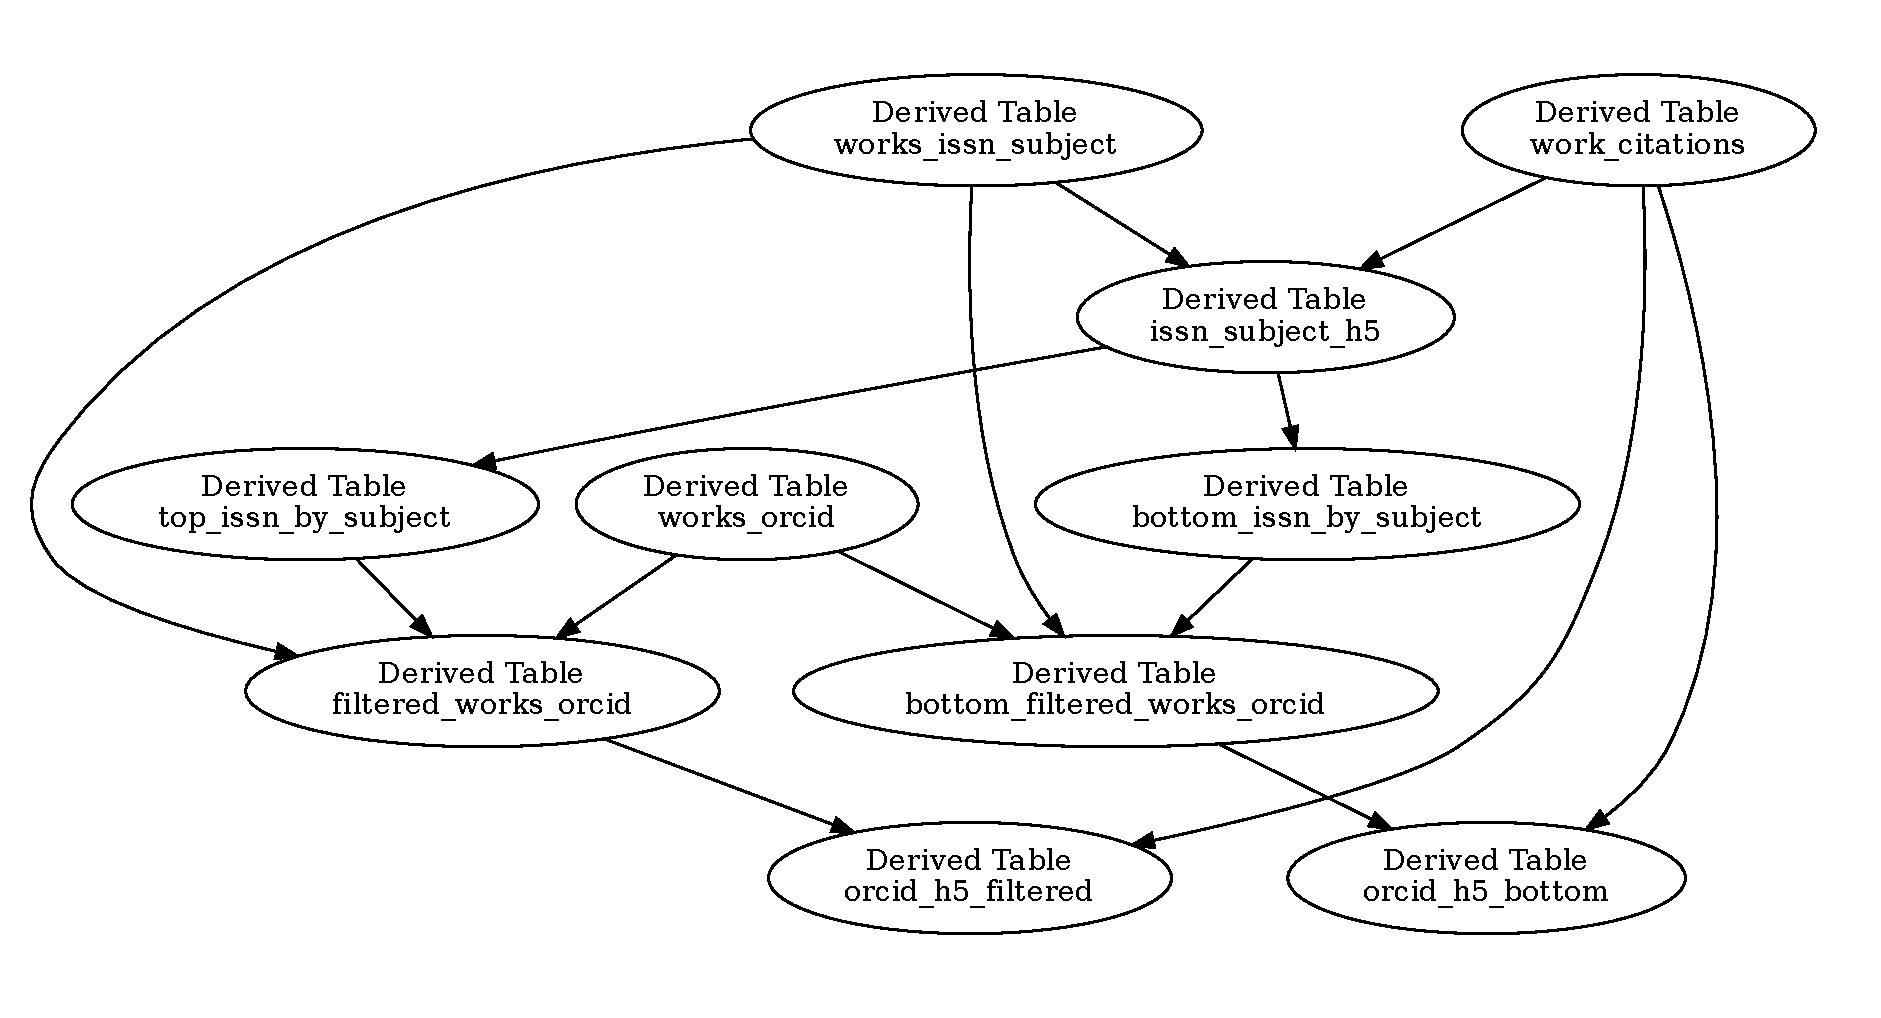
\includegraphics[width=0.8\textwidth]{../figs/h5.pdf}
      \caption{Dependencies of the tables used in the implementation of the Adjusted h-index by filtering the top 20\% and bottom 50\% of journals by subject based on the h5 index.}
      \label{fig:tables}
\end{figure}

Figure \ref{fig:tables2} shows the dependencies of each table for the
implementation of the JIF-adjusted h-index by filtering the top 20\% of
journals by subject based on the Journal Impact Factor (JIF).

\begin{figure}[H]
      \centering
      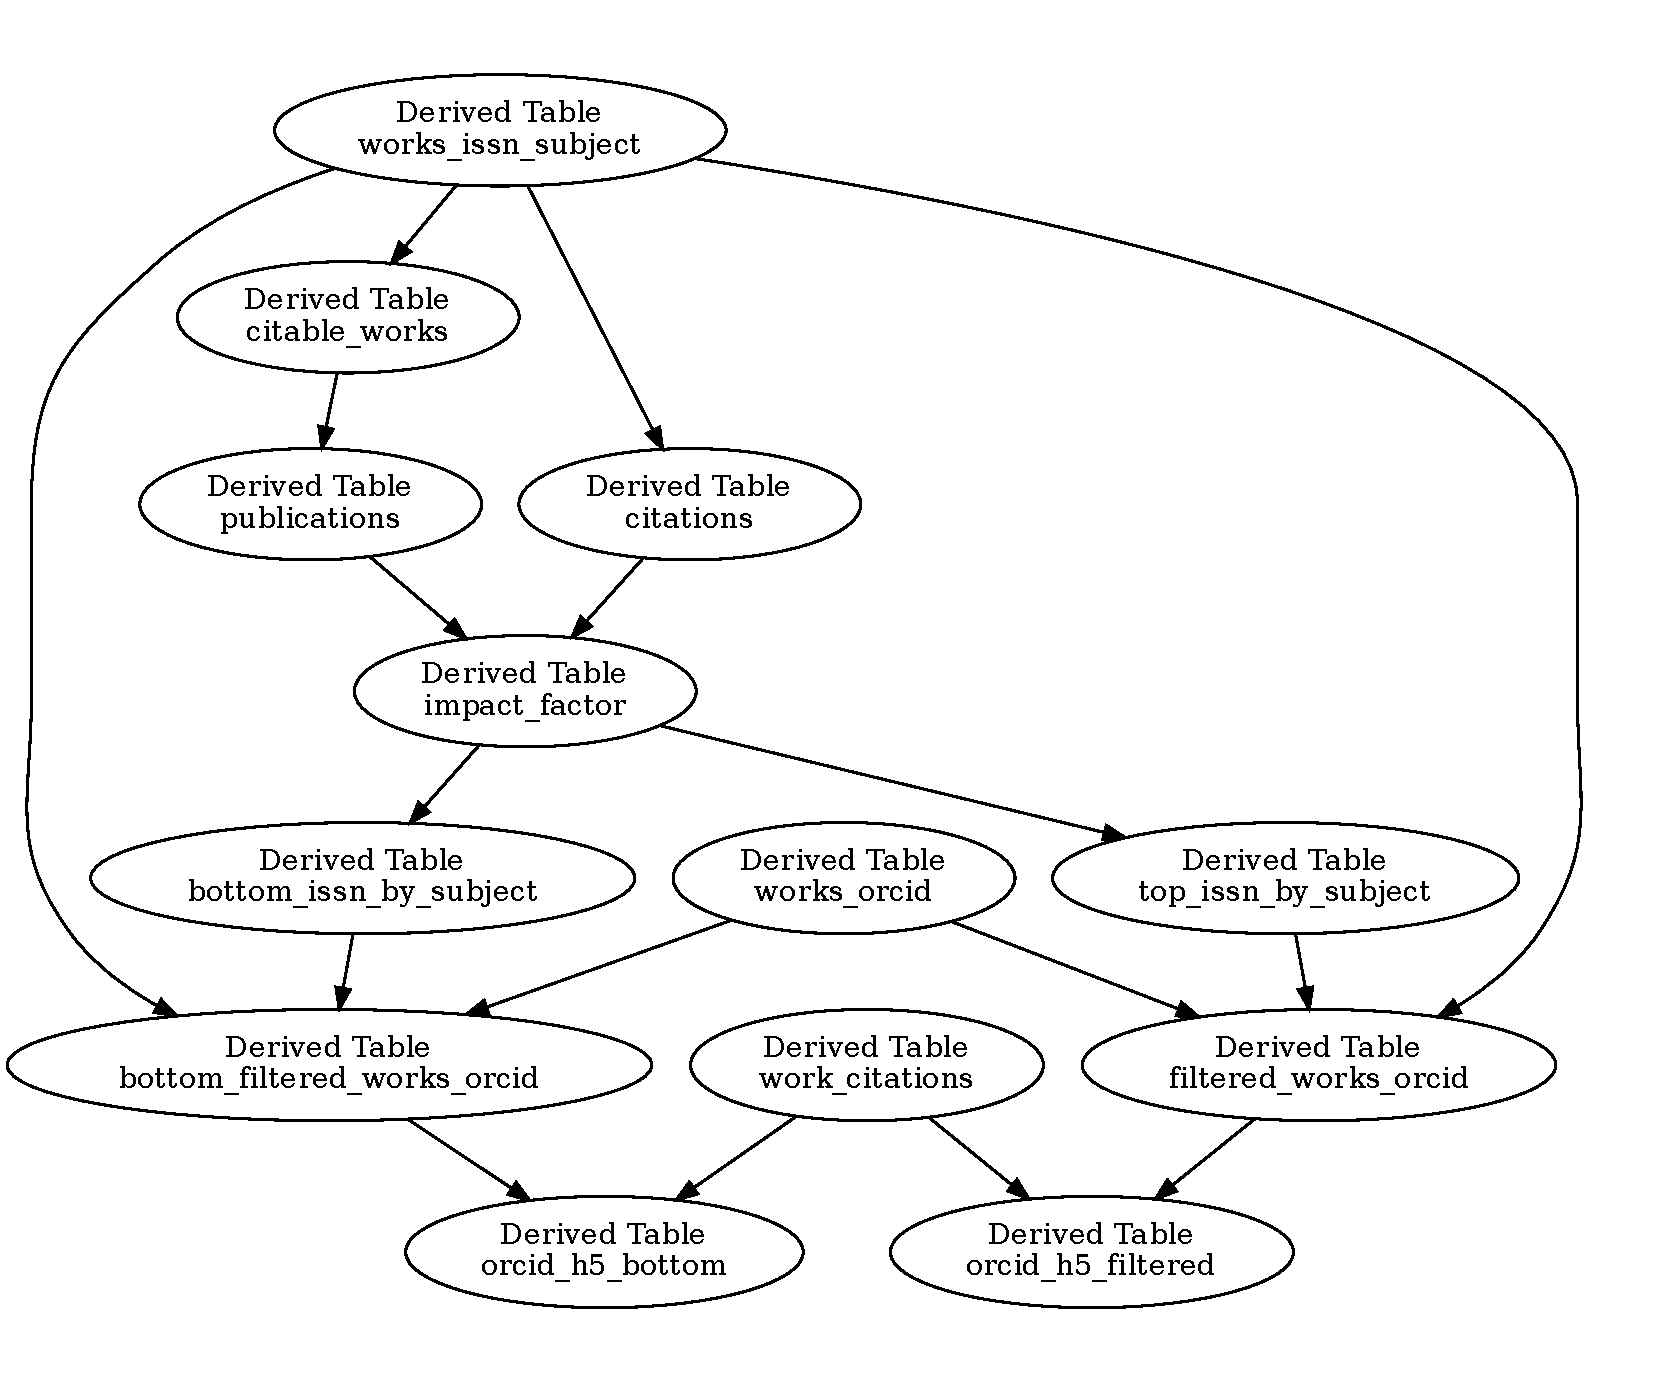
\includegraphics[width=0.8\textwidth]{../figs/impact.pdf}
      \caption{Dependencies of the tables used in the implementation of the JIF-adjusted h-index by filtering the top 20\% and bottom 50\% of journals by subject based on the Journal Impact Factor (JIF).}
      \label{fig:tables2}
\end{figure}

Figure \ref{fig:tables3} shows the dependencies of each table for the
implementation of the EigenFactor-adjusted h-index by filtering the top 20\% of
journals by subject based on the EigenFactor.

\begin{figure}[H]
      \centering
      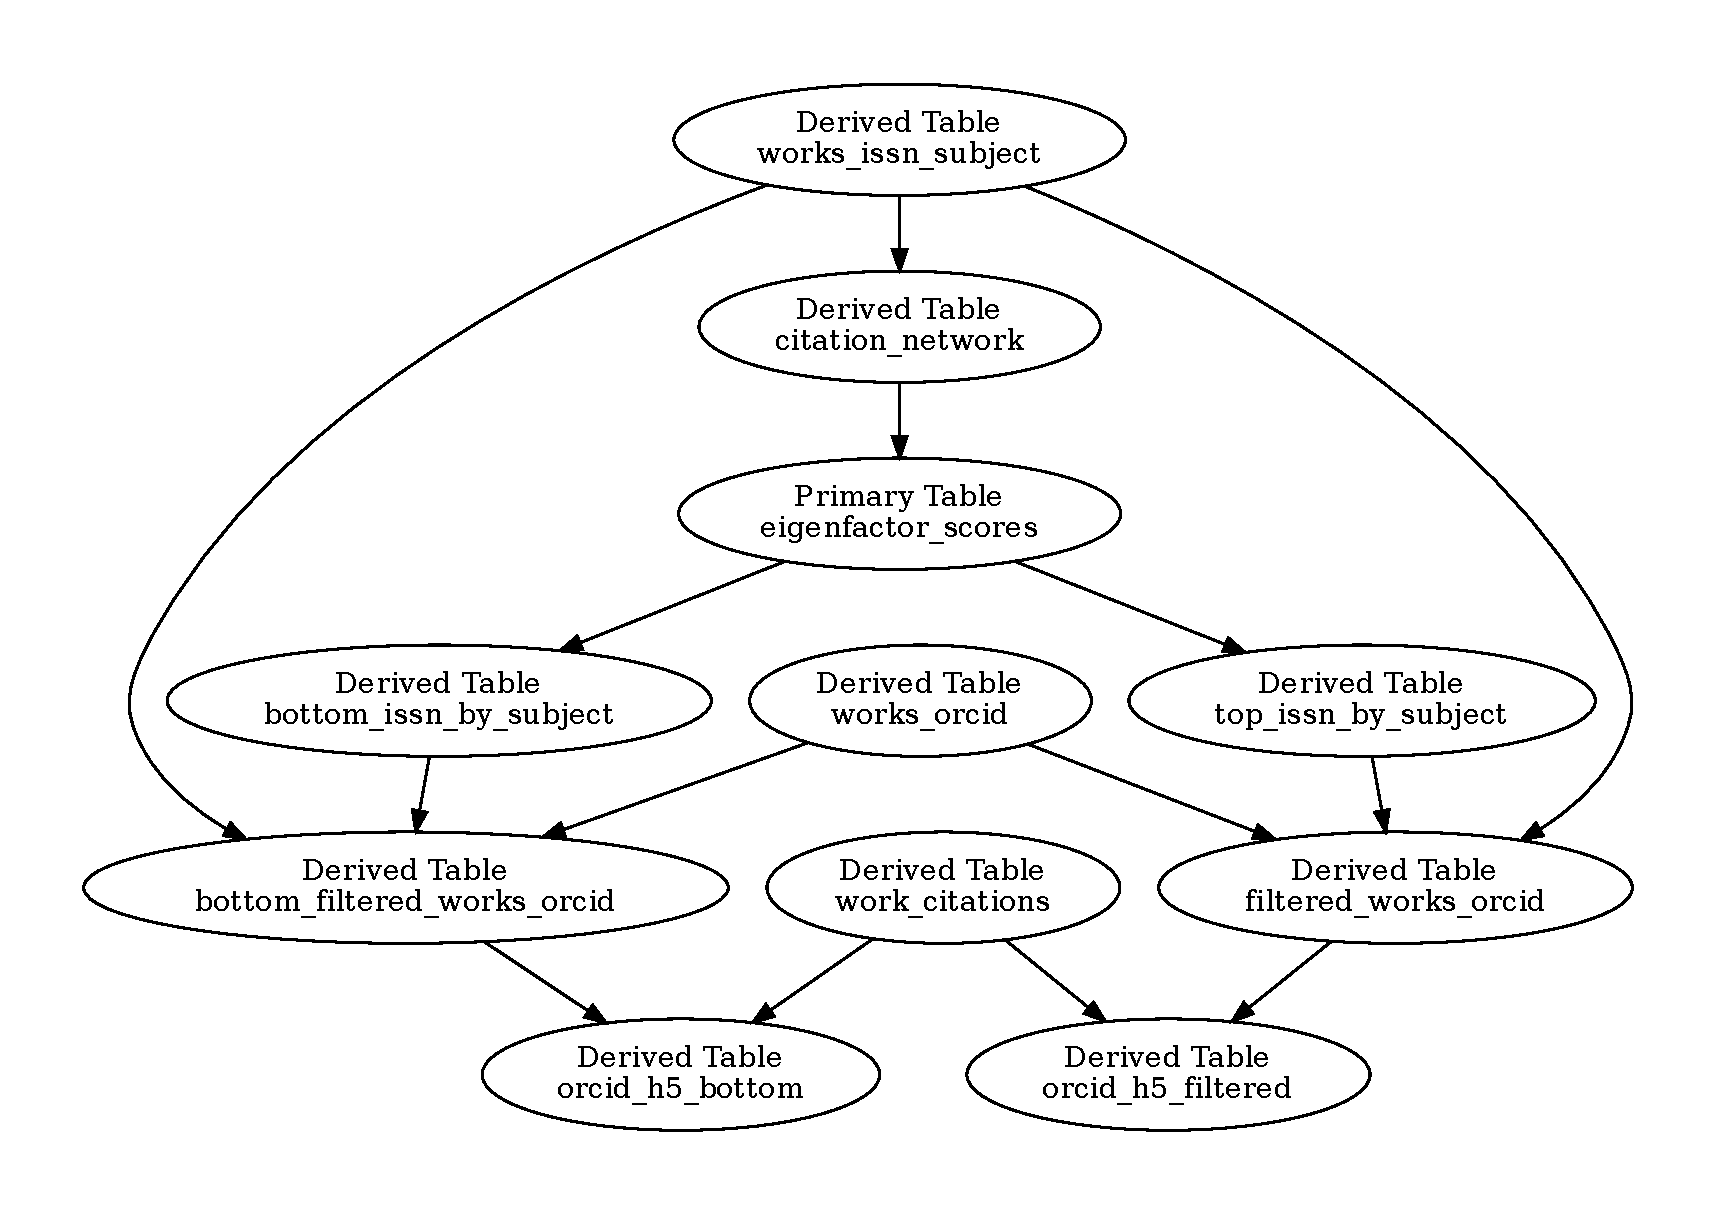
\includegraphics[width=0.8\textwidth]{../figs/eigenfactor.pdf}
      \caption{Dependencies of the tables used in the implementation of the EigenFactor-adjusted h-index by filtering the top 20\% and bottom 20\% of journals by subject based on the EigenFactor.}
      \label{fig:tables3}
\end{figure}

